\documentclass[UTF8,12pt,a4paper]{ctexart}

\usepackage[a4paper,top=24mm,bottom=24mm,left=25mm,right=25mm]{geometry}
\usepackage{amsmath,amssymb}
\usepackage{booktabs,array,tabularx,longtable,multirow}
\usepackage{graphicx,float,caption,subcaption}
\usepackage{siunitx}
\usepackage{xcolor}
\usepackage{fancyhdr}
\usepackage{hyperref}
\usepackage{url}

\graphicspath{{figures/}{../FourBranchRev/output/}{../Localization/output/}}
\hypersetup{
  colorlinks=true,
  linkcolor=blue!55!black,
  urlcolor=blue!60!black,
  pdftitle={分布式相控阵定位系统实测实验报告},
  pdfauthor={王越、杨天宇、杨沛峰}
}
\captionsetup{font=small,labelfont=bf}
\setlength{\parindent}{2em}
\setlength{\parskip}{0.25em}
\setlength{\emergencystretch}{2em}
\renewcommand{\arraystretch}{1.18}

\definecolor{accent}{RGB}{29,78,121}
\definecolor{lightaccent}{RGB}{233,241,248}
\pagestyle{fancy}
\fancyhf{}
\fancyhead[L]{分布式相控阵定位系统实测实验报告}
\fancyhead[R]{2026-09-18}
\fancyfoot[C]{\thepage}
\setlength{\headheight}{15pt}

\newcommand{\code}[1]{\texttt{#1}}
\newcommand{\importantbox}[1]{%
  \begin{center}
  \fcolorbox{accent}{lightaccent}{%
    \begin{minipage}{0.91\textwidth}
      #1
    \end{minipage}}
  \end{center}}

\begin{document}

\begin{titlepage}
  \centering
  \vspace*{18mm}
  {\zihao{2}\bfseries 分布式相控阵使能的物联网设备高精度定位\par}
  \vspace{10mm}
  {\zihao{1}\bfseries 实测实验报告\par}
  \vspace{8mm}
  {\Large 四分支复响应恢复、宽带 AOA 与多站定位验证\par}
  \vfill
  \begin{tabular}{rl}
    项目编号： & 202661066 \\
    项目类型： & 校级 SRTP 创新训练项目 \\
    项目负责人： & 王越 \\
    项目成员： & 王越、杨天宇、杨沛峰 \\
    指导教师： & 范伟 \\
    实测日期： & 2026 年 8 月 29 日 \\
    报告日期： & 2026 年 9 月 18 日 \\
  \end{tabular}
  \vfill
  {\normalsize 本报告仅针对现有实测数据及其计算结果。\par
  Wireless InSite 仿真正在开展，不在本报告中预写尚未形成的结果。\par}
\end{titlepage}

\pagenumbering{Roman}
\begin{abstract}
本实验使用 Anritsu MS46322B 矢量网络分析仪和 32 通道、$8\times4$ 阵元相控阵，在同一信源位置下完成四个阵列位置的 On/Off、Hadamard 和 REV 测量。三种采集方式形成四条分析分支：Branch 1 复数 DFT、Branch 2 On/Off、Branch 3 Hadamard 和 Branch 4 严格功率 REV。Branch 4 在形成 $|Z_{\mathrm{REV}}|^2$ 后完全不再使用 VNA 相位，仅由功率随受控相移的变化恢复阵元相对复响应，再执行宽带 AOA 估计和多站几何定位。

标准 51 频点分析中，Branch 1 与 Branch 4 的阵元复响应相干系数为 0.943，对齐相位均方根误差为 $15.30^\circ$。四条分支的四站定位误差分别为 1.160 m、1.172 m、1.162 m 和 1.122 m，估计位置高度集中，且均表现出相似的 $y$ 方向偏差。进一步枚举 Branch 4 的全部 3--9 次相移观测子集后，共得到 469 种复响应方法和 5159 条定位链。相移观测数增加时，功率 REV 的有效率、复相干和相位误差均稳定改善，但四站定位误差中位数仍保持在约 1.12--1.17 m。

这些结果说明功率 REV 分支没有出现相对于三个复数参考分支的结构性失效，且能够恢复 AOA 所需的主要阵元相对幅相信息。四分支共同出现的绝对偏差更可能由硬件与射频链路误差、尺规和姿态记录误差、未去嵌通道、室内电磁干扰及多径传播等共同作用形成；现有数据只能说明其总体影响，不能唯一分离各误差源。本实验因此验证了功率 REV 到多站定位的路径可行性，但不把约 1.1 m 的结果表述为已经达到亚米级高精度。

\textbf{关键词：}功率 REV；相控阵；到达角；多站定位；Hadamard 编码；实测验证
\end{abstract}

\tableofcontents
\clearpage
\pagenumbering{arabic}

\section{实验目的与报告范围}

本项目希望在不为每个阵元配置独立高精度相位测量链路的条件下，利用多个受控相移状态下的合成功率，恢复阵元相对复响应，并将其用于 AOA 估计和多站三维定位。本次实测报告的目的包括：

\begin{enumerate}
  \item 验证严格功率 REV 能否在不使用 VNA 实测相位的条件下恢复可用于 AOA 的阵元相对复响应；
  \item 使用复数 DFT、On/Off 和 Hadamard 三条参考分支交叉检查功率 REV；
  \item 比较四条分支的单站 AOA、两站/三站/四站定位结果；
  \item 通过全部相移观测子集穷举，判断结论是否依赖某一个特定相移组合；
  \item 根据实测数据如实说明当前系统的精度边界和可能误差来源。
\end{enumerate}

本报告不包含尚在进行中的 Wireless InSite 仿真结果。Wireless InSite 仍是项目需要完成的工作，完成后应作为独立传播仿真层纳入项目总报告；其尚未完成不改变本报告对现有实测数据的统计事实。

\section{实验系统与测量场景}

\subsection{硬件与扫频设置}

实验系统的主要参数见表~\ref{tab:hardware}。

\begin{table}[H]
  \centering
  \caption{实测硬件与采集参数}
  \label{tab:hardware}
  \begin{tabularx}{\textwidth}{>{\bfseries}p{0.25\textwidth}X}
    \toprule
    项目 & 配置 \\
    \midrule
    矢量网络分析仪 & Anritsu MS46322B \\
    阵列控制模块 & Jiexi BCS3085A-32T1-B1，1 入 32 出 APM（32 路输出） \\
    实体阵列 & $4\times8$ 微带贴片天线阵列，共 32 个阵元；本文按 $x$ 方向 8 个、$z$ 方向 4 个记为 $8\times4$ \\
    测量场地 & 实验前方案记录为 A6-409 办公室内及楼道 \\
    DUT/Probe 方案 & 4×8 贴片阵列，Horn/全向天线 \\
    阵元间距 & 行向和列向均为 3.5 cm \\
    工作频段 & 实验前系统方案为 C band 4--8 GHz；本次实际扫频为 4.5--5.5 GHz，中心频率 5.0 GHz \\
    频点数与 IFBW & 2001 点，IFBW 5 kHz \\
    阵面与朝向 & 阵面平行于 $xoz$ 平面，法向朝 $+y$；被测天线朝 $-y$ \\
    校准状态 & 未进行背景相减、逐通道校准和自由空间去嵌 \\
    \bottomrule
  \end{tabularx}
\end{table}

实验前系统框图中，VNA 一端连接 1 入 32 出 APM，APM 通过 32 路 RF chain 分别驱动贴片阵元；VNA 另一端连接待测设备或探头。方案采用一个实体相控阵，通过移动阵列至少两次形成多个观测位置，再执行 AOA 定位。本次实际采集进一步扩展为同一信源下的 Location1--4 四个阵位，并额外保留 Location5 单站数据。

实验前方案列出了 REV 码本、MUSIC 和 Beamforming。该内容反映实验准备阶段的算法选项；本报告的最终数据处理以四分支复响应恢复和宽带非相干 Bartlett AOA 为准，不把方案图中的算法名称误写为本次已经使用的处理方法。

阵元按四个 $z$ 高度层编号，每层包含沿 $x$ 方向排列的 8 个阵元。相对于阵列几何中心，阵元坐标为
\begin{equation}
  x=(r-4.5)\times 0.035\ \mathrm{m},\qquad
  z=(2.5-c)\times 0.035\ \mathrm{m},
\end{equation}
其中 $r=1,\ldots,8$，$c=1,\ldots,4$。

\subsection{多站几何与数据范围}

Location1--4 使用同一信源位置，可组成多站定位闭环。坐标见表~\ref{tab:geometry}，原始记录由厘米统一换算为米。

\begin{table}[H]
  \centering
  \caption{四个阵列位置与信源真值}
  \label{tab:geometry}
  \begin{tabular}{lccc}
    \toprule
    对象 & $x$ (m) & $y$ (m) & $z$ (m) \\
    \midrule
    Location1 阵列中心 & 1.32 & -0.11 & 1.69 \\
    Location2 阵列中心 & 2.42 & -0.11 & 1.69 \\
    Location3 阵列中心 & 0.00 & 0.00 & 1.69 \\
    Location4 阵列中心 & -1.21 & 0.00 & 1.69 \\
    被测信源真值 & 0.00 & 3.09 & 1.50 \\
    \bottomrule
  \end{tabular}
\end{table}

Location1--4 均包含 On/Off、Hadamard 和 REV 数据。Location5 使用另一个信源位置且只有 On/Off 数据，因此只适合作为单站观察，不进入本报告的四站闭环。结果根目录中另有一组场景元数据未闭合的 Hadamard 数据，也不纳入正式统计。

\section{四分支复响应恢复方法}

\subsection{Branch 1：复数 DFT 参考}

REV 测量包含 $0^\circ,45^\circ,\ldots,315^\circ$ 八个唯一相位以及 $360^\circ$ 闭合重复点。Branch 1 对前八个唯一相位下的复数总响应 $Z(\phi_k)$ 提取一阶 DFT 分量：
\begin{equation}
  H_{\mathrm{B1}}=\frac{1}{8}\sum_{k=1}^{8}Z(\phi_k)e^{-j\phi_k}.
\end{equation}
该分支使用 VNA 相位，与 Branch 4 共用同一套原始 REV 采集，是最直接的同源复数参考。

\subsection{Branch 2：On/Off 直接测量}

每次只开启一个目标阵元，其余阵元设置为高衰减状态，直接测得每个阵元的复数 S21，形成 $H_{\mathrm{Direct}}$。该方法直观，但会受到开关隔离度、逐状态漂移和测量链路误差影响，因此作为参考而不是无误差真值。

\subsection{Branch 3：Hadamard 正交编码}

32 个阵元同时工作并依次施加 32 组 $0^\circ/180^\circ$ 正交码字。令 Hadamard 码矩阵为 $C$、阵元响应为 $h$、码字测量为 $Y$，则
\begin{equation}
  Y=Ch,\qquad H_{\mathrm{B3}}=\frac{C^{\mathrm H}Y}{32}.
\end{equation}
该分支可获得编码复响应，但也可能受到多通道同时工作时的非线性、移相误差、互耦和漂移影响。

\subsection{Branch 4：严格功率 REV}

Branch 4 首先对 REV 原始复数总响应取模平方：
\begin{equation}
  P(\phi)=|Z_{\mathrm{REV}}(\phi)|^2.
\end{equation}
从此步骤开始，算法不再访问 VNA 相位。功率模型写为
\begin{equation}
  P(\phi)=D+2\operatorname{Re}\!\left\{C e^{j\phi}\right\},
  \qquad C=B^*H,
\end{equation}
其中 $B$ 为其余阵元形成的背景场，$H$ 为目标阵元响应。对直流项、余弦项和正弦项进行最小二乘拟合后，根据二次根关系恢复相对响应 $H/(B+H)$。该响应允许存在一个全阵列公共复比例；公共增益和公共相位零点不改变阵元间相对波前，因此不影响 AOA。

\importantbox{\textbf{分支隔离原则：}Branch 4 的定位输入只能来自 $|Z_{\mathrm{REV}}|^2$ 重算得到的 $H_{\mathrm{RevPower}}$。VNA 复相位只用于 Branch 1 和离线对照，不能回流到 Branch 4。历史 MAT 文件中的旧 $H_{\mathrm{RevPower}}$ 曾引入复数背景相位，本报告不使用该旧字段。}

\section{比较指标、AOA 与定位方法}

\subsection{复响应一致性}

同一位置、同一频点的两组 32 阵元响应记为 $a$ 和 $b$。仅允许使用一个对全部阵元共有的复标量
\begin{equation}
  q=\frac{a^{\mathrm H}b}{a^{\mathrm H}a}
\end{equation}
对齐整体增益和相位零点。之后计算复相干系数、对齐相位 RMSE、复数 NMSE 和幅度 NRMSE。该操作不包含逐阵元调参。

\subsection{宽带 AOA}

正式定位在 4.5--5.5 GHz 内均匀选取 51 个频点，采用宽带非相干 Bartlett 方向余弦搜索。每个频点允许独立的公共复增益，将归一化空间匹配得分跨频点平均后得到方向向量。该实现适用于当前单次复响应观测，不把单快拍秩一数据误写为可稳定区分子空间的 MUSIC 结果。

\subsection{多站几何定位}

两站定位取两条空间方向直线最近点的中点；三站和四站定位最小化估计点到全部方向线的垂距平方和，并用 Huber IRLS 降低异常射线影响。每个结果同时检查射线参数是否向前。

射线 RMS 仅反映多条射线的内部交汇一致性，不等于相对真实坐标的定位误差。带有共同方向偏差的射线可以在错误位置紧密交汇，因此报告始终同时给出真值误差。

\section{标准四分支结果}

\subsection{复响应一致性}

表~\ref{tab:agreement}为标准 51 频点分析中，先对频点取中位数、再对四个阵位取中位数的结果。

\begin{table}[H]
  \centering
  \caption{四分支两两复响应一致性}
  \label{tab:agreement}
  \begin{tabular}{lrrrr}
    \toprule
    分支对 & 相干系数 & 相位 RMSE & 复数 NMSE & 幅度 NRMSE \\
    \midrule
    B1--B2 & 0.819 & $40.28^\circ$ & -4.91 dB & 0.384 \\
    B1--B3 & 0.971 & $14.65^\circ$ & -12.46 dB & 0.161 \\
    B1--B4 & 0.943 & $15.30^\circ$ & -9.97 dB & 0.257 \\
    B2--B3 & 0.827 & $37.40^\circ$ & -5.12 dB & 0.370 \\
    B2--B4 & 0.737 & $45.91^\circ$ & -3.41 dB & 0.477 \\
    B3--B4 & 0.913 & $22.44^\circ$ & -7.96 dB & 0.294 \\
    \bottomrule
  \end{tabular}
\end{table}

Branch 1 与 Branch 4 的同源对照最关键。Branch 4 主动丢弃 VNA 相位后仍取得 0.943 的相干系数和 $15.30^\circ$ 的相位 RMSE，说明功率 REV 已恢复 AOA 所需的主要阵元相对幅相结构。Branch 2 与其他分支的复响应一致性相对较弱，但后续 AOA 和定位仍与其他分支接近，提示绝对定位结果还受到分支之外的共同系统因素影响。

\begin{figure}[H]
  \centering
  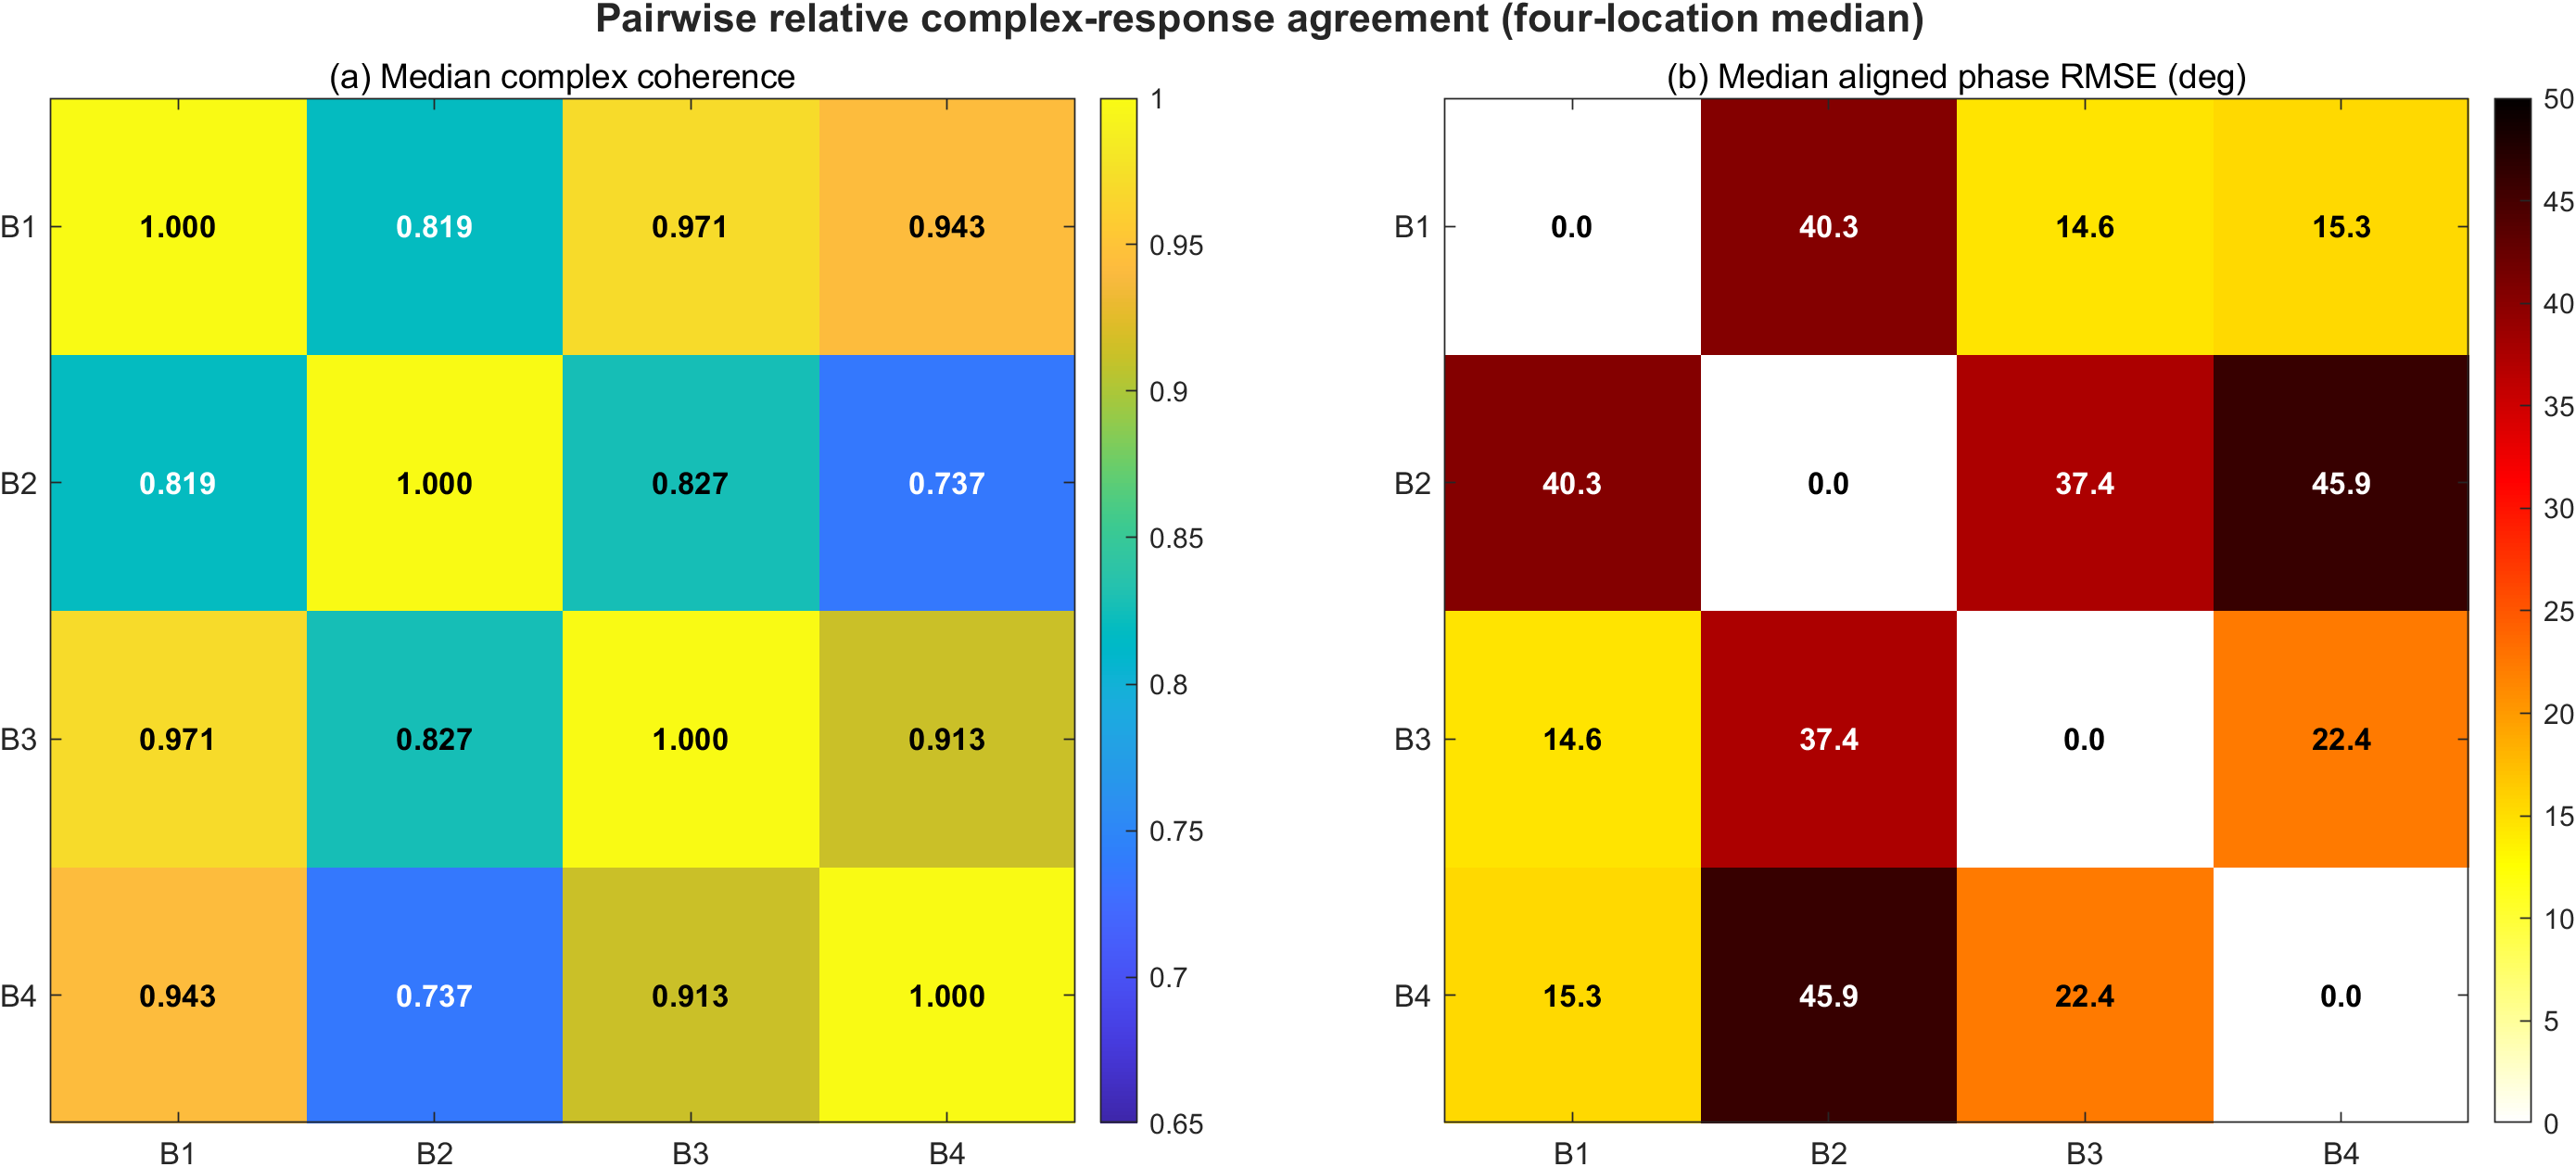
\includegraphics[width=0.98\textwidth]{response_agreement_matrix.png}
  \caption{四分支相对复响应的一致性矩阵。对角线表示同一分支；非对角元素为四个阵位的中位统计。}
  \label{fig:agreement}
\end{figure}

\subsection{单站 AOA}

四条分支在每个阵位的角误差非常接近，见表~\ref{tab:doa}. Location2 在所有分支中均为最大误差，Location4 均为最小误差。这种“误差主要随阵位变化、而不是随分支变化”的现象，是共同环境与几何误差的重要证据。

\begin{table}[H]
  \centering
  \caption{四分支单站 AOA 角误差（单位：度）}
  \label{tab:doa}
  \begin{tabular}{lrrrr}
    \toprule
    分支 & Location1 & Location2 & Location3 & Location4 \\
    \midrule
    B1 复数 DFT & 12.16 & 16.69 & 8.37 & 5.16 \\
    B2 On/Off & 11.75 & 16.93 & 9.42 & 5.44 \\
    B3 Hadamard & 12.07 & 16.73 & 8.71 & 5.31 \\
    B4 功率 REV & 11.75 & 16.25 & 8.37 & 5.16 \\
    \bottomrule
  \end{tabular}
\end{table}

\subsection{四站定位}

真实信源坐标为 $(0,3.09,1.50)$ m。四站正式结果见表~\ref{tab:fourstation} 和图~\ref{fig:localization}。

\begin{table}[H]
  \centering
  \caption{四分支四站定位结果}
  \label{tab:fourstation}
  \begin{tabular}{lrrrrr}
    \toprule
    分支 & $x$ (m) & $y$ (m) & $z$ (m) & 真值误差 (m) & 射线 RMS (m) \\
    \midrule
    B1 复数 DFT & -0.264 & 1.962 & 1.557 & 1.160 & 0.269 \\
    B2 On/Off & -0.259 & 1.949 & 1.571 & 1.172 & 0.283 \\
    B3 Hadamard & -0.259 & 1.958 & 1.554 & 1.162 & 0.277 \\
    B4 功率 REV & -0.263 & 2.001 & 1.564 & 1.122 & 0.263 \\
    \bottomrule
  \end{tabular}
\end{table}

\begin{figure}[H]
  \centering
  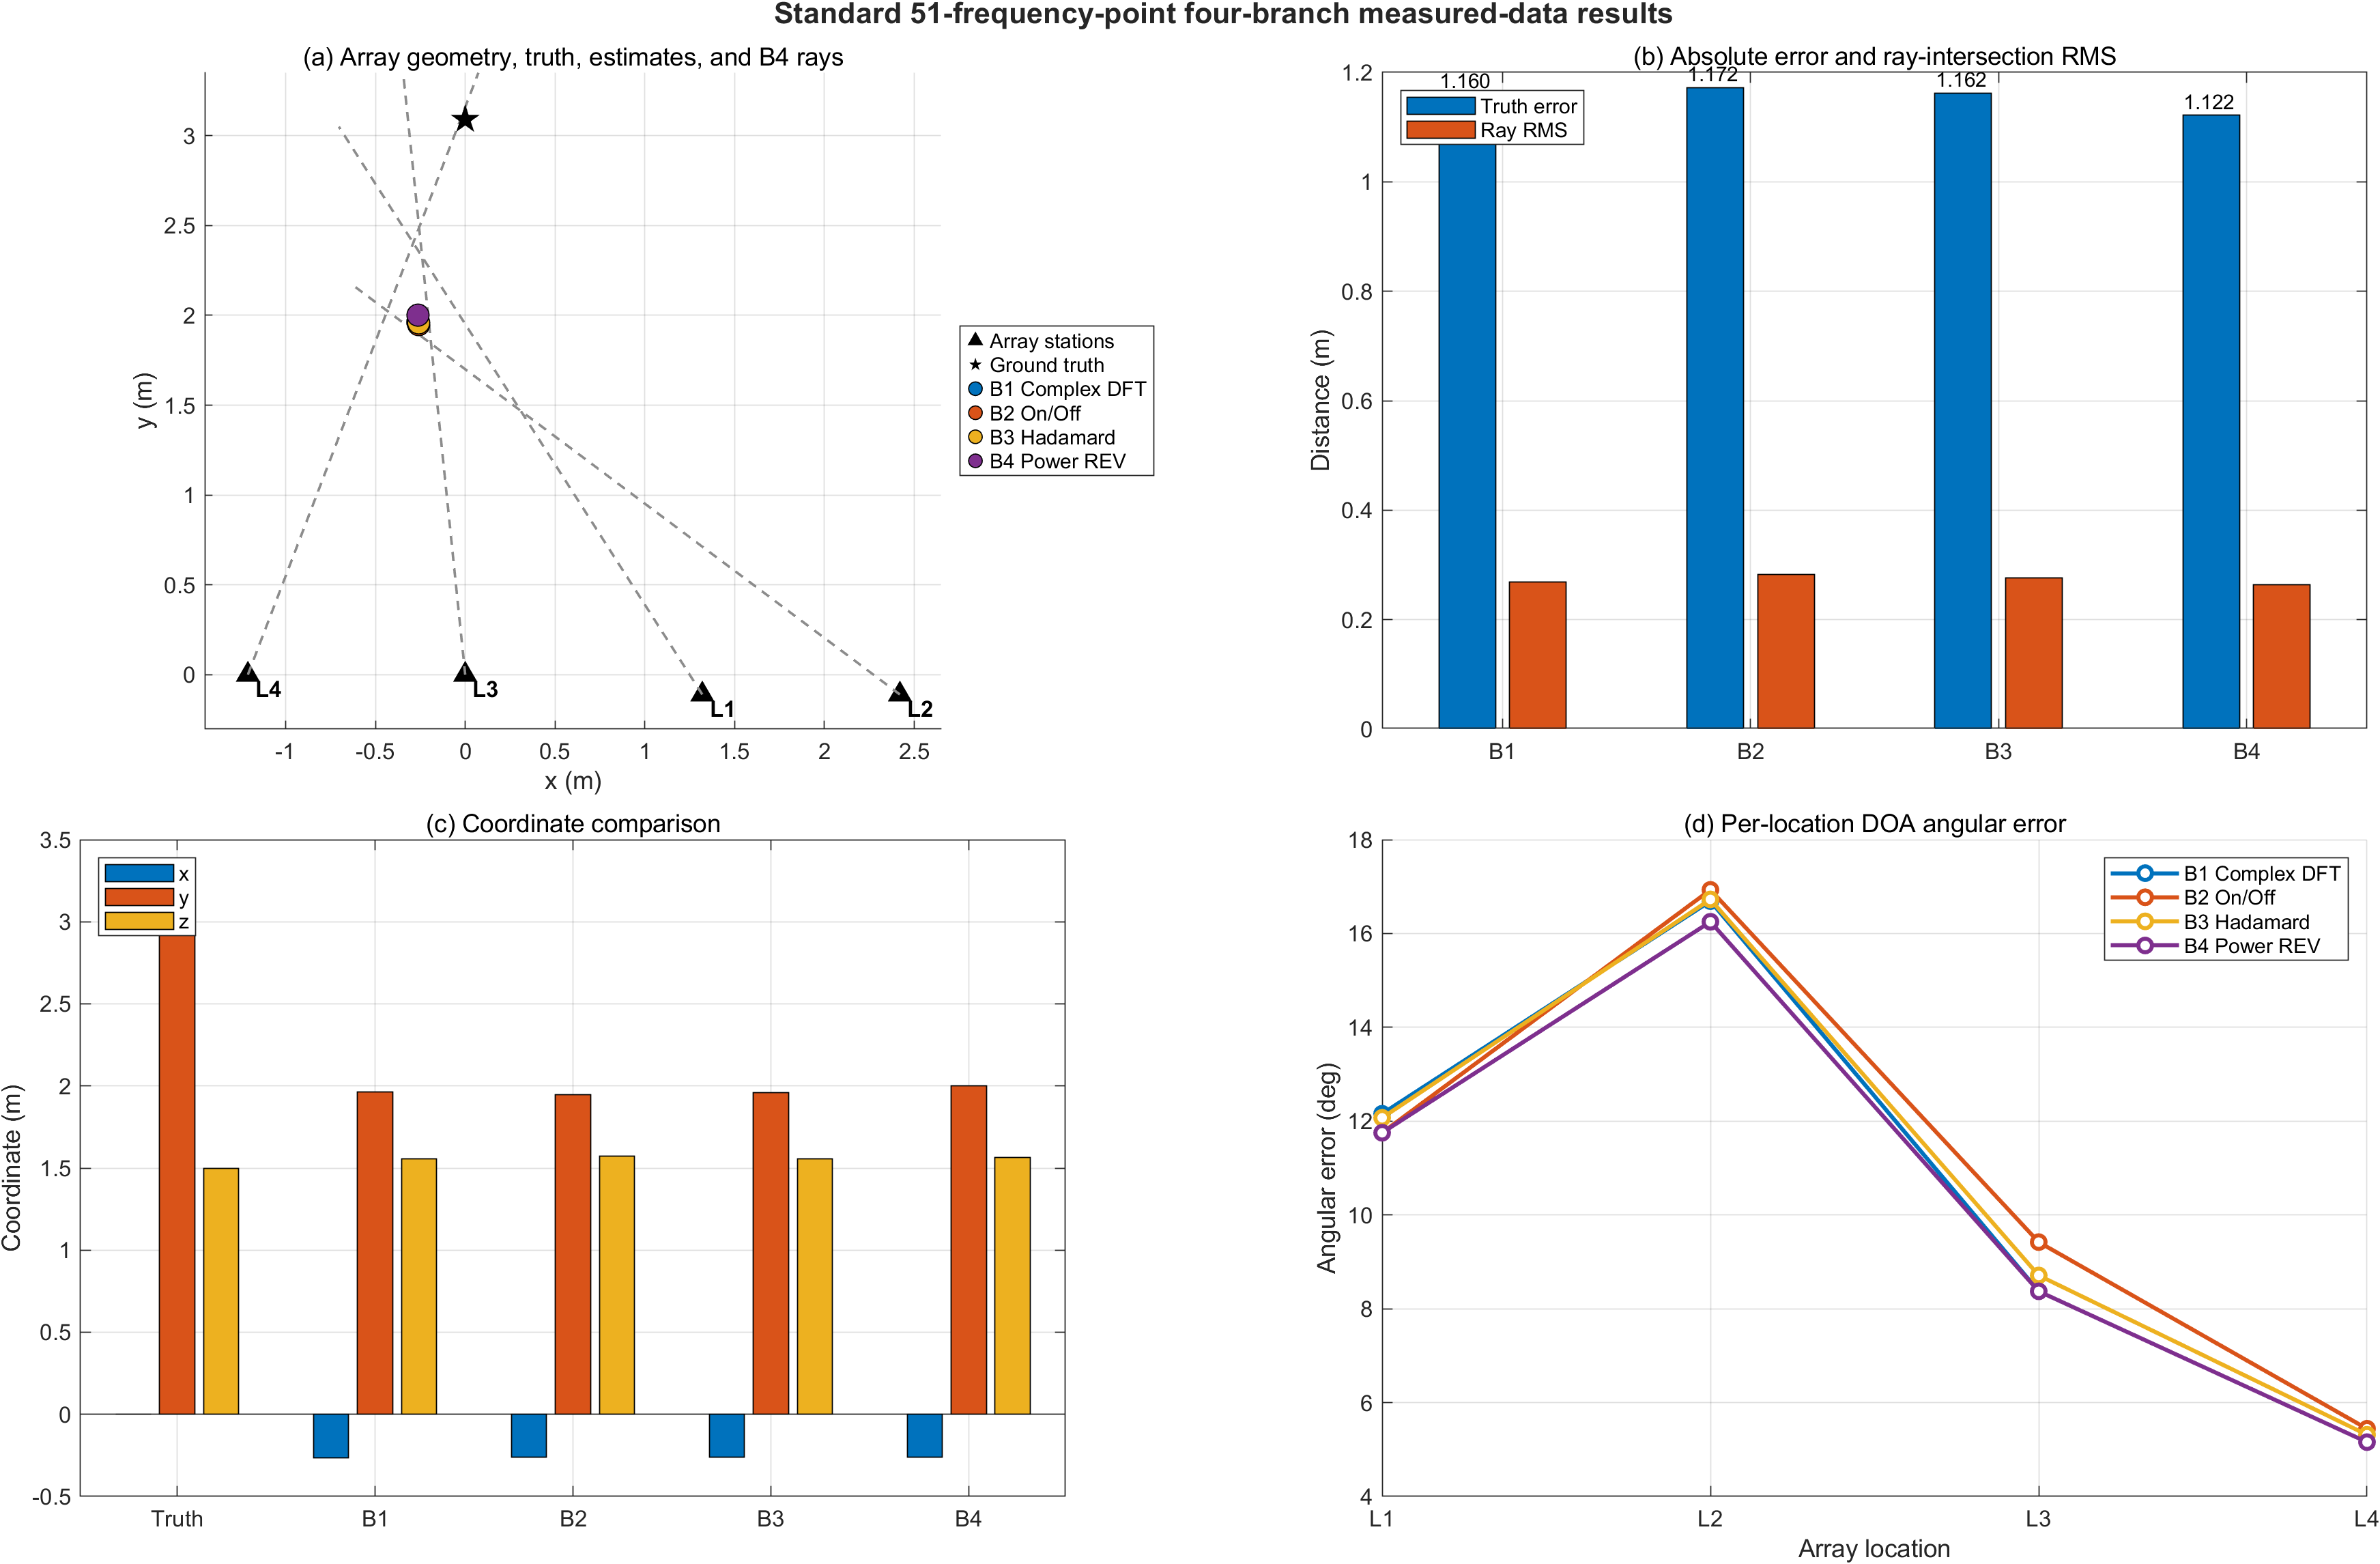
\includegraphics[width=\textwidth]{four_branch_localization.png}
  \caption{标准 51 频点四分支实测定位对照。四条分支的估计位置高度集中，且均相对真值表现出主要沿 $y$ 方向的共同偏差。}
  \label{fig:localization}
\end{figure}

四条分支的 $y$ 估计均位于约 1.95--2.00 m，而真值为 3.09 m；$x$ 和 $z$ 估计也高度接近。Branch 1 与 Branch 4 的三维估计坐标相差约 4 cm，远小于它们各自约 1.1 m 的真值误差。因此，当前绝对偏差不是 Branch 4 独有，不能解释为功率 REV 算法发生结构性错误。

标准闭环还包含每个分支的 6 个两站组合、4 个三站组合和 1 个四站组合，共 44 条定位结果。两站、三站、四站的分支间趋势一致；增加站数可以提高约束数量，但不能自动消除多个阵位共有的方向偏差。

\section{Branch 4 全相移子集穷举}

\subsection{穷举空间与完整性}

从九次实测观测中任选 3--9 次，Branch 4 方法数为
\begin{equation}
  \sum_{k=3}^{9}\binom{9}{k}=466.
\end{equation}
加上 Branch 1--3 各一种正式方法，共 469 种复响应方法。每种方法运行 6 个两站、4 个三站和 1 个四站定位，因此共有
\begin{equation}
  469\times 11=5159
\end{equation}
条完整定位链。为保证所有方法公平比较，穷举统一使用 21 个等间隔频点；该口径与标准闭环的 51 频点结果分开报告。

实际输出包括 1876 条单站 AOA 和 5159 条定位链。其中 5082 条获得数值定位；7 个三观测子集同时包含 $0^\circ$、$360^\circ$ 和一个其他相位，只有两个唯一名义相位，功率设计矩阵秩为 2，导致对应 77 条定位链不可恢复。数值定位中另有 84 条两站/三站结果未通过全部射线向前检查，四站结果全部通过。

\subsection{相移观测数对响应与定位的影响}

表~\ref{tab:exhaustive}中的 3--9 表示四个阵位各自使用的 REV 相移观测数，不是参与定位的阵位数。每个相移子集仍然在 Location1--4 分别恢复响应并进行四站定位。

\begin{table}[H]
  \centering
  \caption{Branch 4 全子集结果汇总}
  \label{tab:exhaustive}
  \resizebox{\textwidth}{!}{%
  \begin{tabular}{rrrrrrr}
    \toprule
    观测数 & 子集数 & 可恢复子集 & 有效率中位数 & 对 B1 相干 & 相位 RMSE & 四站误差中位数 \\
    \midrule
    3 & 84 & 77 & 83.48\% & 0.703 & $50.33^\circ$ & 1.123 m \\
    4 & 126 & 126 & 90.40\% & 0.844 & $33.27^\circ$ & 1.157 m \\
    5 & 126 & 126 & 93.27\% & 0.893 & $26.17^\circ$ & 1.162 m \\
    6 & 84 & 84 & 94.87\% & 0.921 & $21.43^\circ$ & 1.163 m \\
    7 & 36 & 36 & 96.06\% & 0.938 & $18.66^\circ$ & 1.165 m \\
    8 & 9 & 9 & 96.95\% & 0.948 & $16.62^\circ$ & 1.166 m \\
    9 & 1 & 1 & 97.62\% & 0.959 & $13.57^\circ$ & 1.168 m \\
    \bottomrule
  \end{tabular}}
\end{table}

\begin{figure}[H]
  \centering
  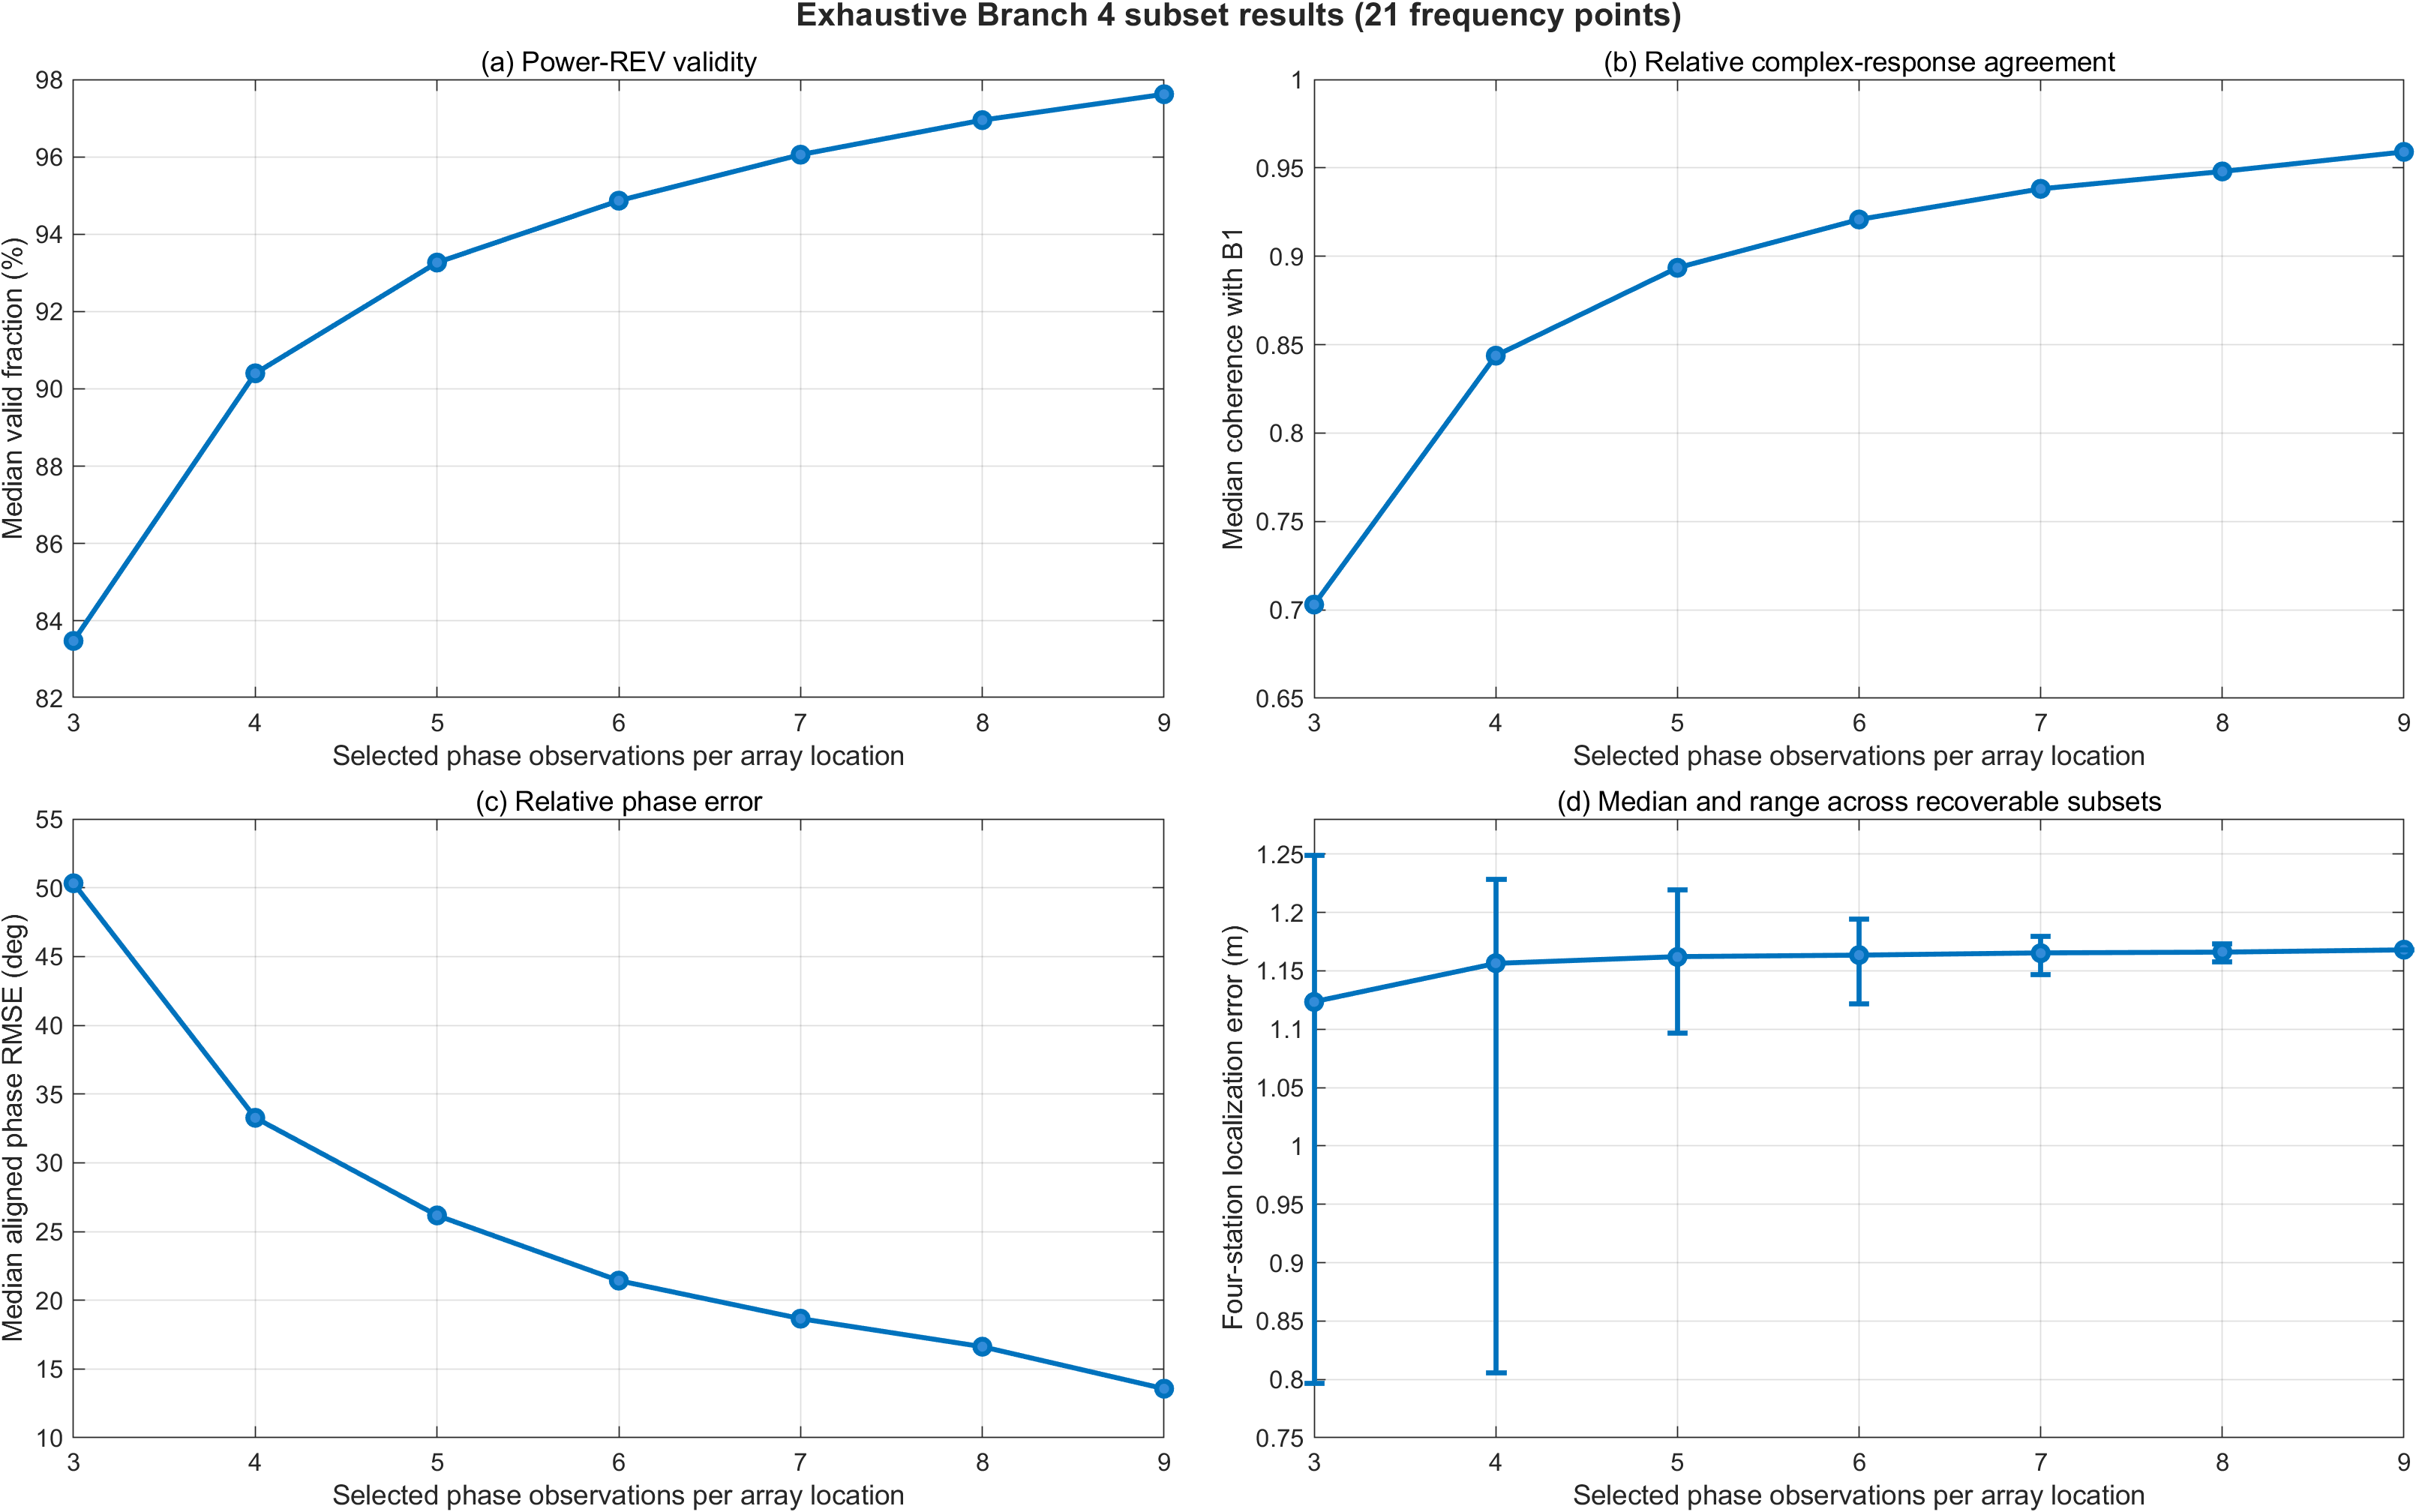
\includegraphics[width=\textwidth]{phase_observation_summary.png}
  \caption{Branch 4 相移观测子集穷举结果。随着观测数增加，复响应恢复持续改善，但四站定位误差没有同步接近真值。}
  \label{fig:phasecount}
\end{figure}

\begin{figure}[H]
  \centering
  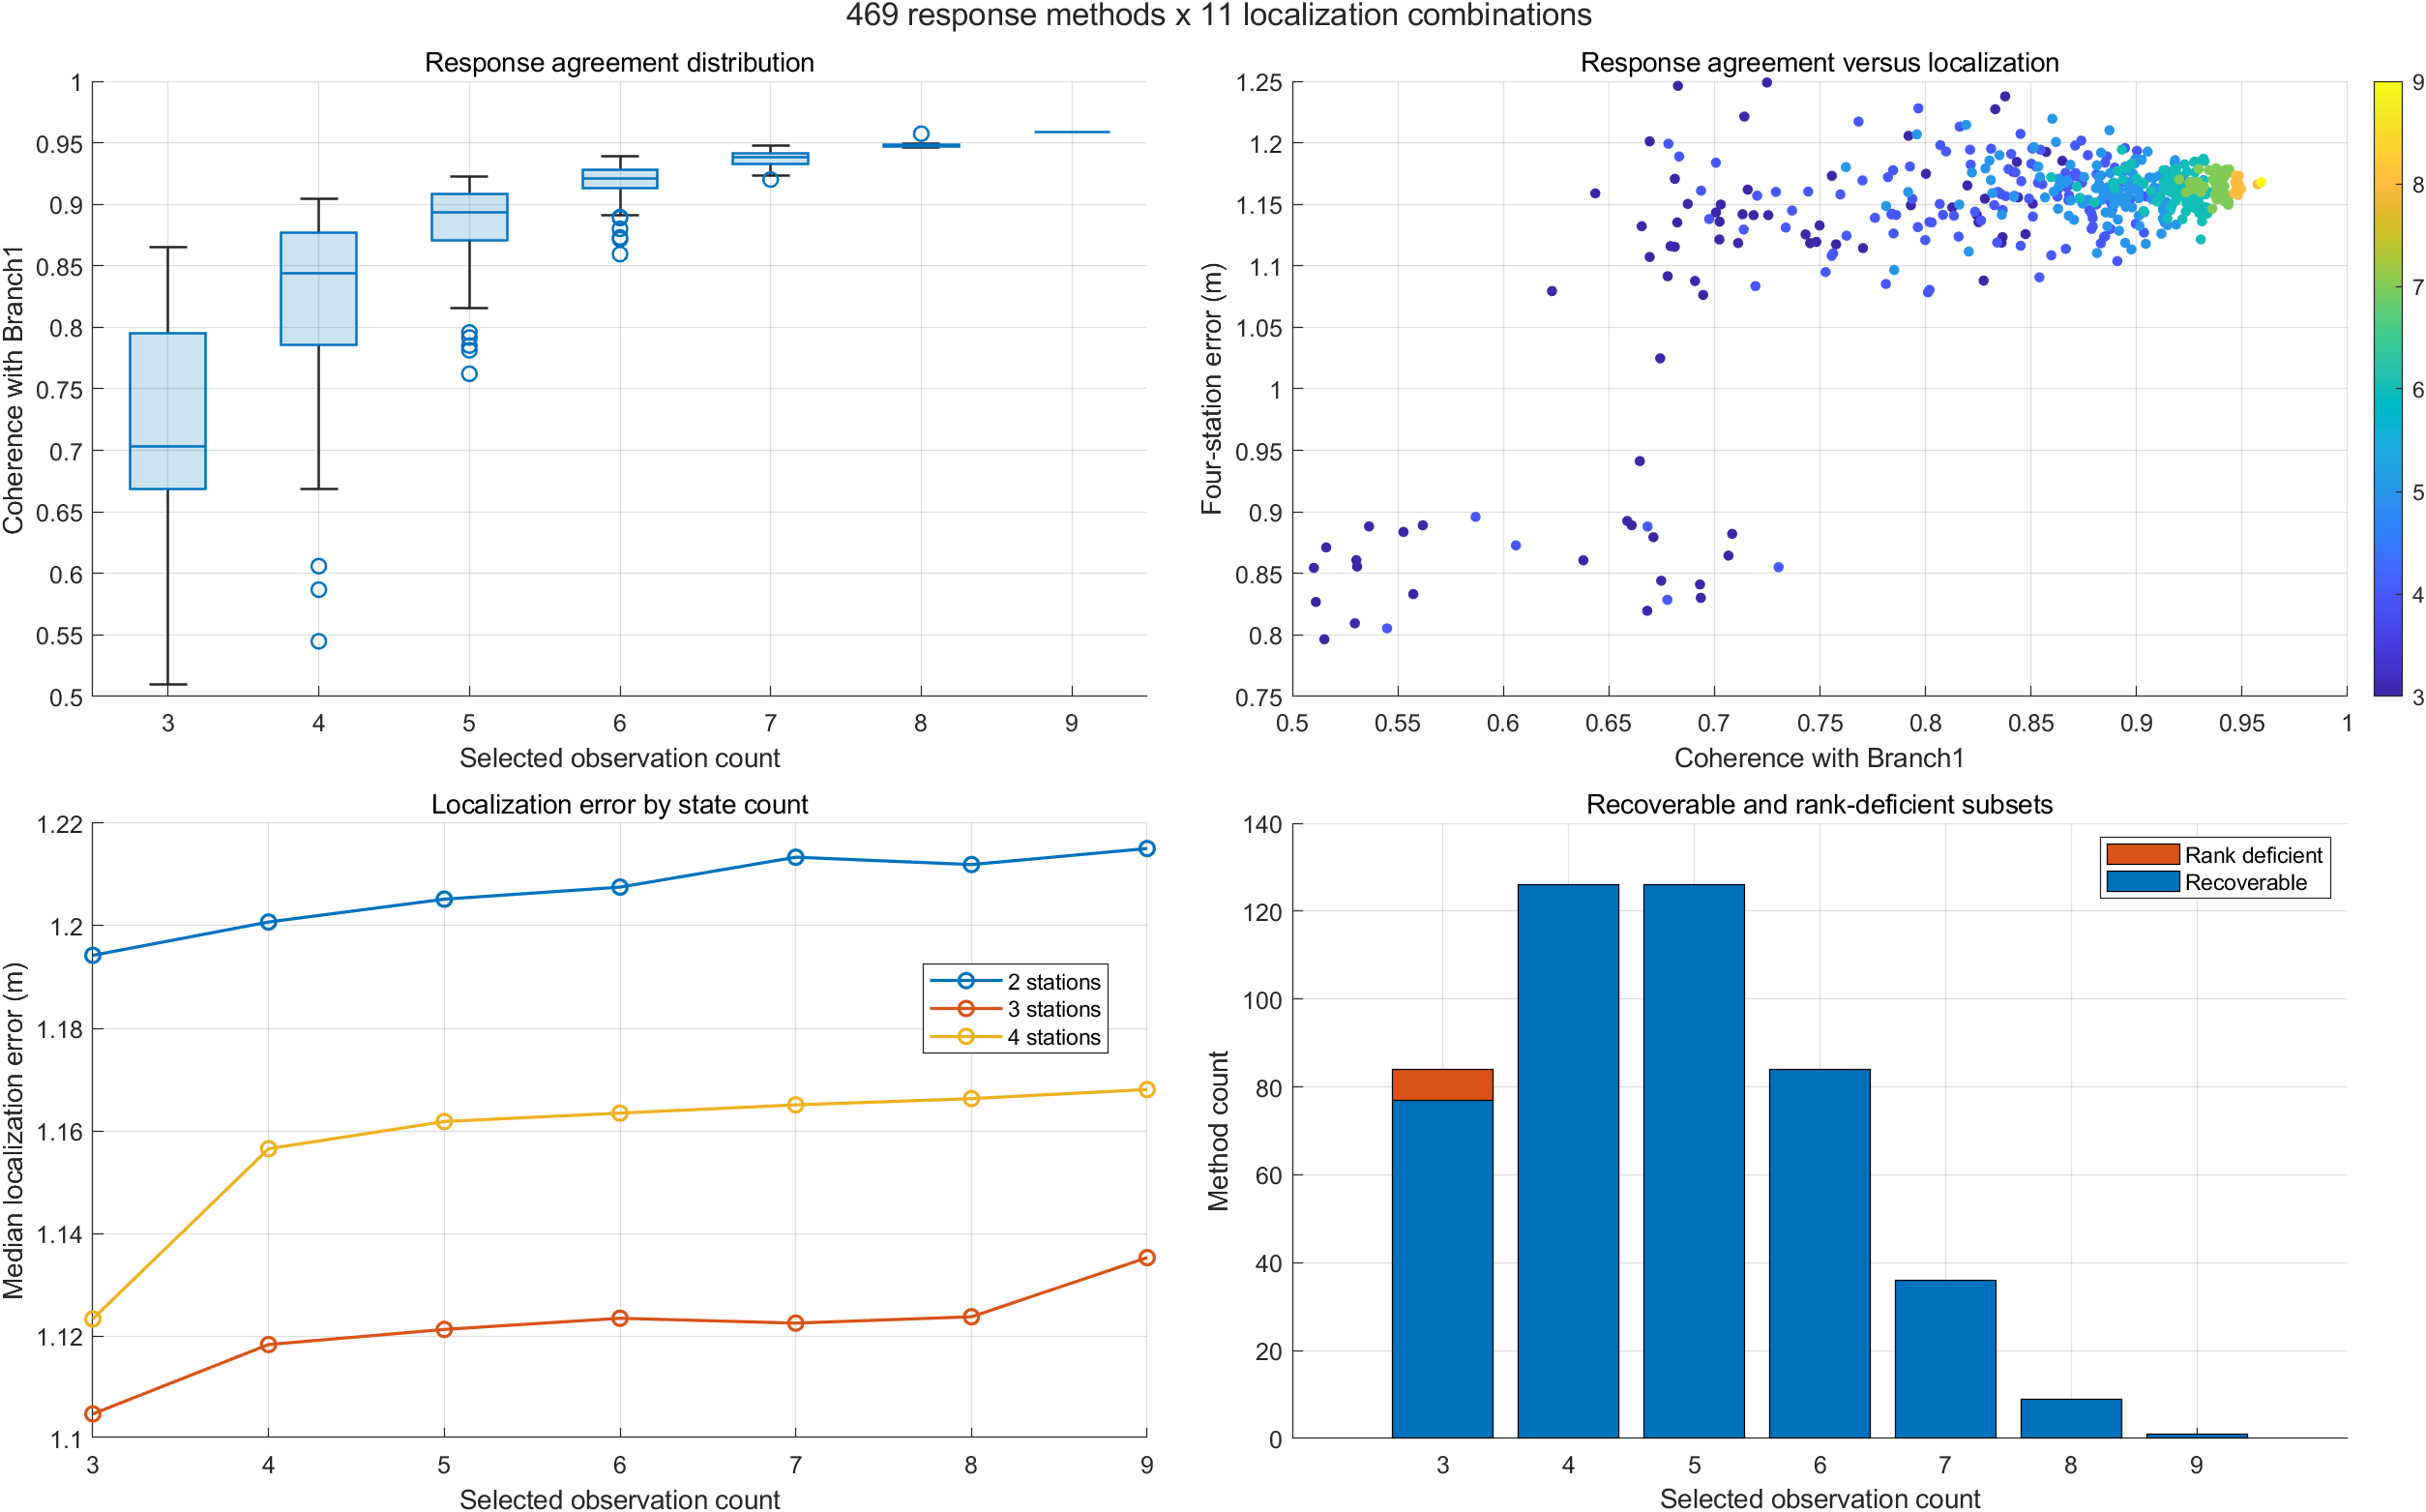
\includegraphics[width=\textwidth]{exhaustive_comparison.png}
  \caption{469 种响应方法与 5159 条定位链的总体分布。少量低观测数子集出现较小真值误差，但其复响应一致性较差，属于误差偶然抵消，不能作为未知信源条件下的相移选择规则。}
  \label{fig:exhaustive}
\end{figure}

观测数由 3 增加到 9 后，有效率、相干系数和相位 RMSE 均明显改善，说明更多功率观测能够稳定提高 REV 复响应质量。然而四站定位误差中位数仍约为 1.12--1.17 m，未随复响应质量提高而逼近真值。这进一步排除了“当前约 1.1 m 偏差主要由 Branch 4 相移观测不足导致”的解释。

\section{误差分析与讨论}

\subsection{数据能够直接支持的判断}

现有数据能够直接支持以下判断：

\begin{enumerate}
  \item 四条分支通过不同方式获得阵元复响应，但四站估计位置高度集中；
  \item 严格功率 REV 与同源复数 DFT 具有较高复响应一致性；
  \item 四条分支在每个阵位的 AOA 误差趋势相近，误差大小主要随阵位变化；
  \item 增加 Branch 4 相移观测数显著改善复响应，却没有消除共同定位偏差；
  \item 因此功率 REV 算法没有表现出独立于参考分支的结构性问题。
\end{enumerate}

\subsection{可能的共同误差来源}

结合实验记录，约 1.1 m 的共同偏差可能来自以下因素的叠加：

\begin{itemize}
  \item \textbf{硬件与射频链路误差：}32 路通道的增益、相位、开关隔离度和移相误差未进行逐通道校准；线缆、连接器和控制模块也会引入公共或通道相关误差。
  \item \textbf{尺规与坐标记录误差：}阵列中心、信源位置和高度由现场尺规记录，几何中心与电磁相位中心可能不完全一致。
  \item \textbf{阵列姿态误差：}分析使用理想阵面法向和水平/竖直方向；实际偏航、俯仰和滚转的小误差会在数米传播距离上放大为明显位置偏差。
  \item \textbf{电磁干扰与室内多径：}墙面、地面、设备和人员反射会改变阵元间相对波前；不同阵位的多径结构不同，可解释 Location2 的角误差持续偏大。
  \item \textbf{未去嵌通道与背景场：}当前数据没有背景相减和自由空间去嵌，最终结果代表“仪器--阵列--环境”整体链路，而不是纯算法误差。
  \item \textbf{频率选择性与时间漂移：}宽带平均可以降低单一频点异常的影响，但不能完全消除采集期间的链路漂移和频率相关多径。
\end{itemize}

以上因素均具有工程合理性，但当前只有一次场景下的四阵位数据，没有独立的姿态复测、逐通道标定、背景测量或跨日期重复实验，因此不能从现有结果中唯一估计各误差源的贡献。报告应使用“可能来自共同系统误差”的表述，而不能把偏差确定归因于某一个因素。

\subsection{结果边界}

本实验验证的是技术路径可行性和多分支一致性，不是亚米级指标的最终证明。约 1.1 m 是当前未校准实测系统的端到端精度表现。射线 RMS 约 0.26--0.28 m 小于真值误差，说明多条射线能够相对一致地交汇在一个带有共同偏差的位置，这也证明仅使用射线交汇残差不足以评价绝对定位精度。

\section{结论}

\importantbox{\textbf{核心结论：}复数 DFT、On/Off、Hadamard 和严格功率 REV 四条分支给出了高度相近的 AOA 与多站定位结果。Branch 4 在完全不使用 VNA 相位的条件下，仍恢复出与复数参考高度相关的阵元相对幅相结构；因此现有实测未发现功率 REV 算法的结构性问题。四分支共同约 1.1 m 的绝对偏差更可能是硬件链路、尺规与姿态记录、未去嵌通道以及室内电磁干扰和多径传播等共同系统误差的结果。}

具体结论如下：

\begin{enumerate}
  \item Branch 1 与 Branch 4 的标准复响应相干系数为 0.943，对齐相位 RMSE 为 $15.30^\circ$；
  \item 四条分支四站定位误差为 1.122--1.172 m，估计位置高度集中；
  \item 469 种复响应方法和 5159 条定位链的穷举结果证明结论不依赖单一相移子集或单一站数组合；
  \item 更多相移观测能提高功率 REV 的恢复质量，但不能消除四分支共有的绝对定位偏差；
  \item 当前结果应表述为“功率 REV 到多站定位的路径可行，实测绝对精度受现有系统不确定性限制”，不应表述为已经达到亚米级高精度。
\end{enumerate}

\clearpage
\section{复现入口与数据文件}

标准四分支闭环入口为：
\begin{verbatim}
cd('Experiment')
analysis = run_closed_loop_analysis;
\end{verbatim}

469 种方法全子集穷举入口为：
\begin{verbatim}
cd('Experiment')
results = run_exhaustive_comparison;
\end{verbatim}

本报告附图由以下脚本根据冻结 CSV 结果生成：
\begin{verbatim}
cd('Experiment/report')
generate_report_figures;
\end{verbatim}

关键数据文件包括：
\begin{itemize}
  \item \path{FourBranchRev/output/response_pair_metrics.csv}：四分支响应一致性；
  \item \path{Localization/output/doa_results.csv}：标准单站 AOA；
  \item \path{Localization/output/localization_2_3_4_stations.csv}：标准 44 条定位结果；
  \item \path{Localization/output/exhaustive_full_pipeline.csv}：5159 条完整定位链；
  \item \path{Localization/output/exhaustive_group_summary.csv}：按分支与相移观测数汇总。
\end{itemize}

\end{document}
